En esta secci\'on, presentaremos los resultados obtenidos en los experimentos
utilizando lo definido en la secci\'on de desarrollo.

Se buscaron analizar en cada fuente tres tipos de redes segun su escala, es
decir redes pequeña, mediana y gran escala. Estas redes fueron
una hogareña, de unas oficinas, de un laboratorio de una Universidad.

En cada captura se almaceno todo los paquetes que se transmitieron
por la red con el sniffer desarollado como se menciono
previamente. Luego analizados automaticamente por el otro programa `analy\_data`
para producir los graficos que se presentan a continuación.

\subsection{Nodos distinguidos}

En cada experimento se analizaron las dos fuentes de información y se definió
un criterio para distinguir un nodo de cada red. Este criterio consta en que
será distinguido el simbolo con mas probabilidad de ocurrir o equivalentemente
el simbolo que tenga menor información.

Para la fuente $S_2$ una de las hipotesis es que estos nodos "distinguidos" son
nodos especiales como routers, access points, etc. dado que estos participan
en la mayor parte de las comunicaciones con la red como con el exterior.
Por lo cual esto nos daría un método (no 100\% confiable debido a casos
atípicos) de determinar los router en una red.

Otra de las hipotesis que se presenta es que una red \textit{cableada} será
mas "compresible" que una \textit{wireless}. Para esto se mostraron el
cociente de la $\frac{H(S)}{H_{MAX}(S)}$ como se desarrollo en TODO: CITA
y se los comparo entre el mismo tipo de fuente de los distintos experimentos.

\subsection{Descripción de los Gráficos}

En cada experimentación se generaron tres tipos de resultados/graficos.

\begin{itemize}
	\item Un gráfico que muestra una representación tipo torta de la fuente, esto es, la probabilidad de ocurrencia de cada simbolo.
	\item Un gráfico tipo histograma que muestra para cada símbolo la información de este. Este grafico cuenta además con una barra
	horizontar que muestra donde se situa la Entropía de la fuente (en color naranja) y otra barra similar que muestra donde
	se situa la Entropía maxima que podria tener la fuente.
	\item Un gráfico con la topologia de los mensajes de la red. Donde los nodos son \textbf{MAC} address y las
	aristas representan un paquete de un nodo a otro
\end{itemize}

\subsection{Red hogareña}

\subsubsection{Fuente Unicast-Multicast}

 Lo siguiente corresponde a la experimentacion realizada para la fuente Unicast-Multicast en una red WiFi domestica.
 
\hspace*{-1.5cm}
 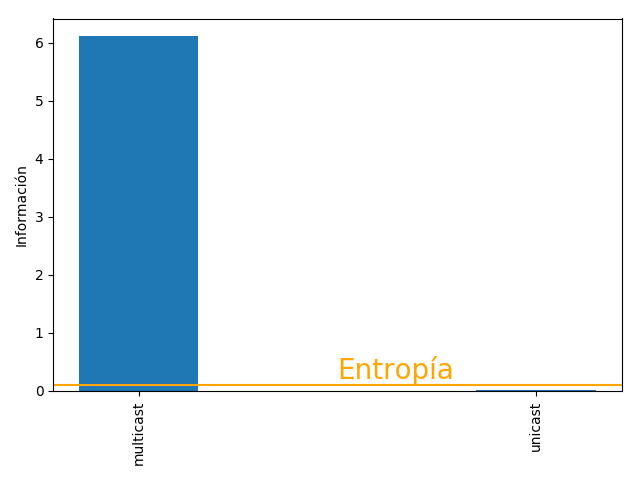
\includegraphics[scale=0.6]{../plots/mauro_s1_informacion.png}
 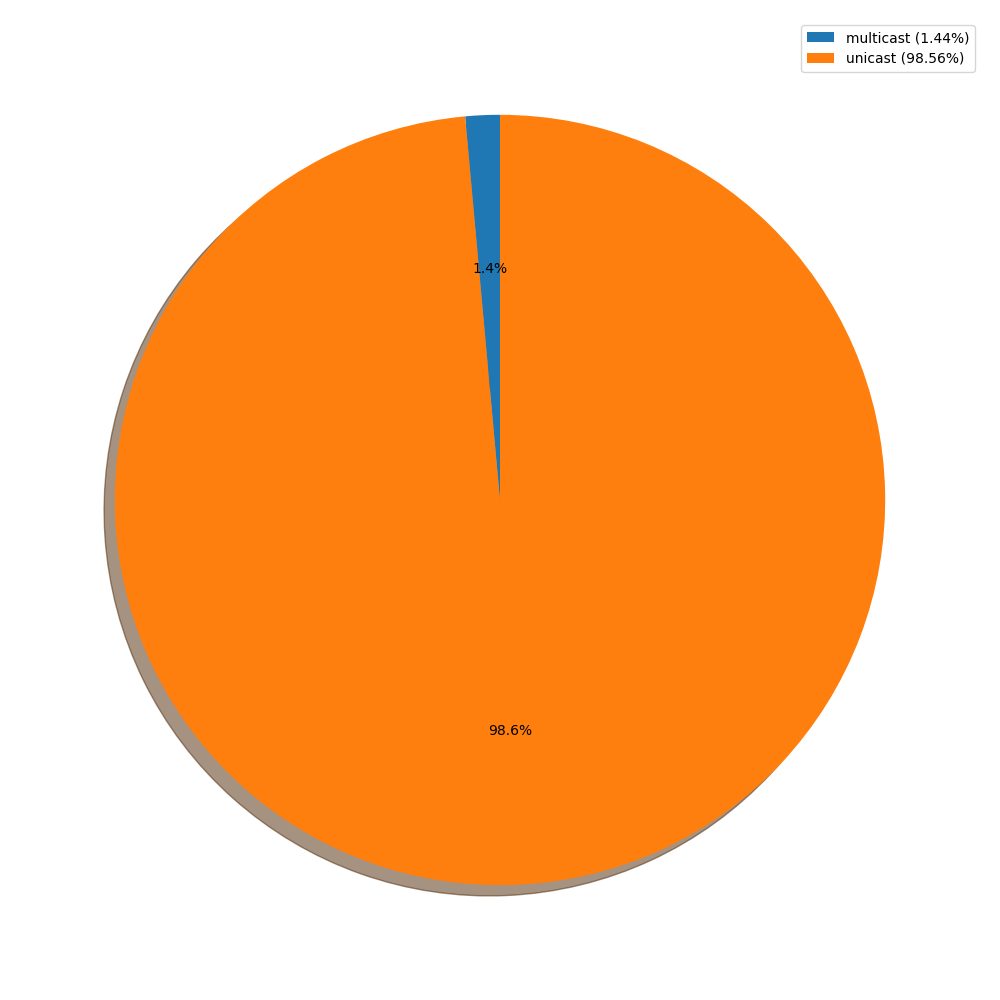
\includegraphics[scale=0.4]{../plots/mauro_s1_probabilidades.png}

 Como podemos ver los resultados obtenidos muestran una alta concentración de paquetes \textit{multicast} por sobre los \textit{unicast}. En concecuencia la entropía cae abruptamente, ya que como explicamos ésta se maximiza cuando la distribución de las probabilidades de cada símbolo es equitativa, y baja a medida que nos alejamos de ello. Nuestra primera impresion era que los paquetes \textit{unicast} iban a predominar en la captura, sin embargo esto no sucedió. Es posible que esto se deba a que la placa de red del dispositivo en el cual se tomó la muestra no hayan entrado en modo promiscuo, en consecuencia el \textit{sniffer} solo llego a capturar los paquetes cuyo destino era dicho dispositivo (y no todos los \textit{unicast} transmitidos en la red). Por el contrario los \textit{multicast} enviados por cualquier dispositivo de la red se pudieron seguir escuchando sin ningun tipo de censura.
 
\subsubsection{Fuente ARP}

\hspace*{-1.5cm}
 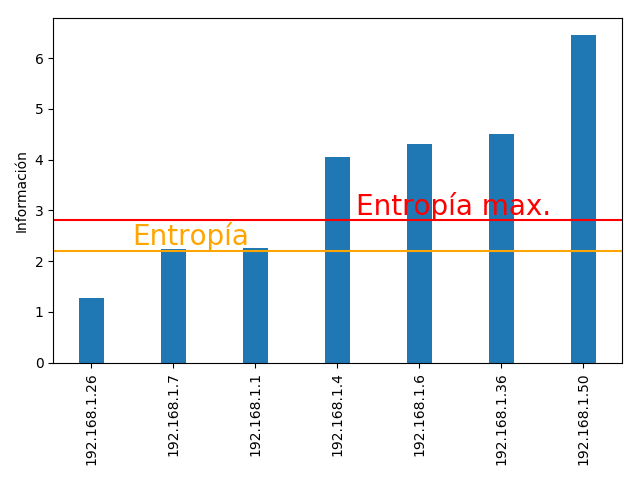
\includegraphics[scale=0.6]{../plots/mauro_s2_informacion.png}
 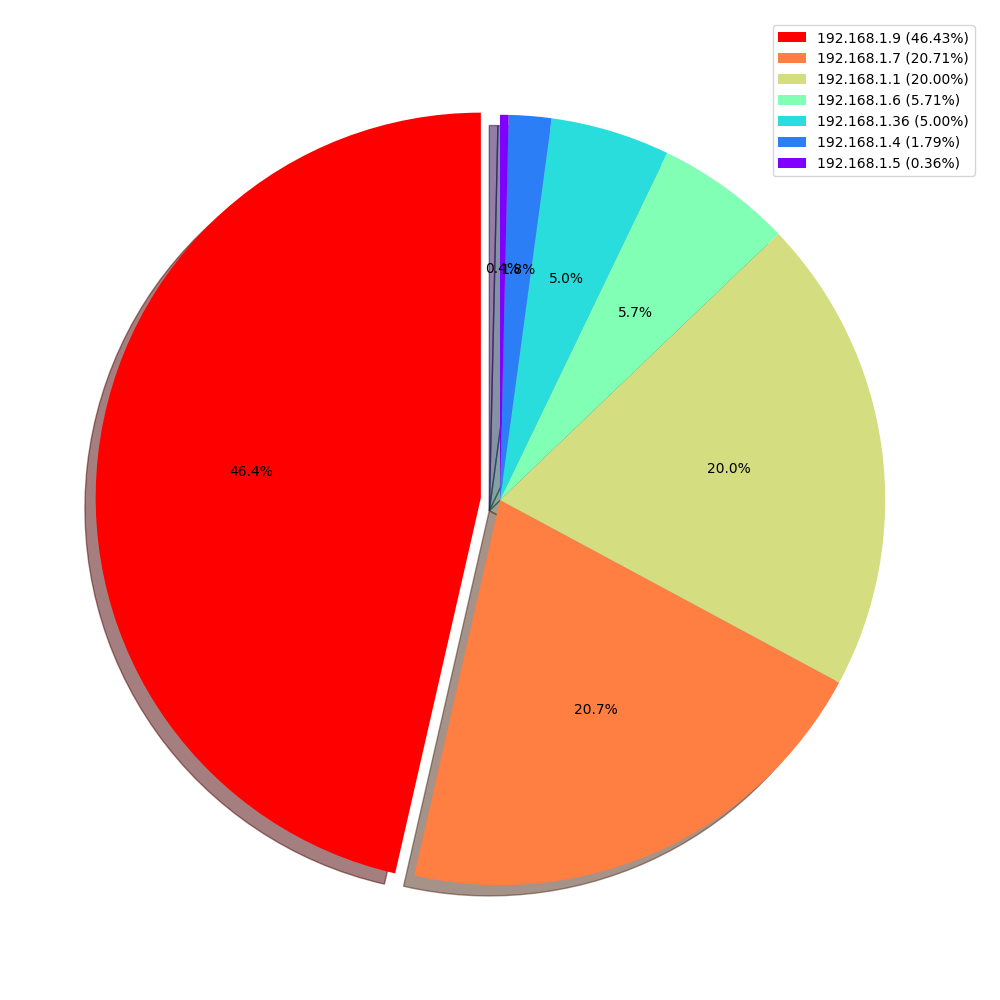
\includegraphics[scale=0.4]{../plots/mauro_s2_probabilidades.png}

\subsubsection{Topolog\'ia de la Red}
\begin{center}
 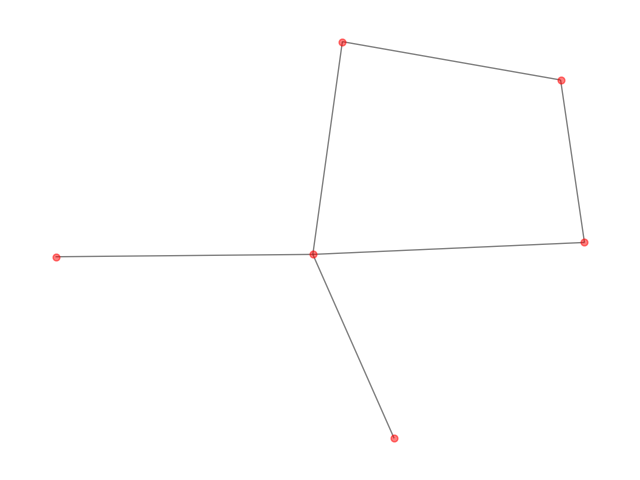
\includegraphics[scale=0.6]{../plots/mauro_s2_topologia.png}
\end{center}

\subsection{\emph{Red del Trabajo}}

En esta caso se analizo una red cableada de mediana escala, 
que consta de 6 oficinas con varias computadoras de escritorio (Desktop) totalizando
una cantidad de 29 estaciones. Además en cada oficina se encuentra un switch que conecta todas
las PCs de esta. La captura que se tomó fue de una hora para 
poder obtener estadísticamente suficiente precision en las medidas y que estas no sean
alteradas por posibles `outliers`.

\subsubsection{Fuente Unicast-Multicast}

\begin{figure}
\centering
 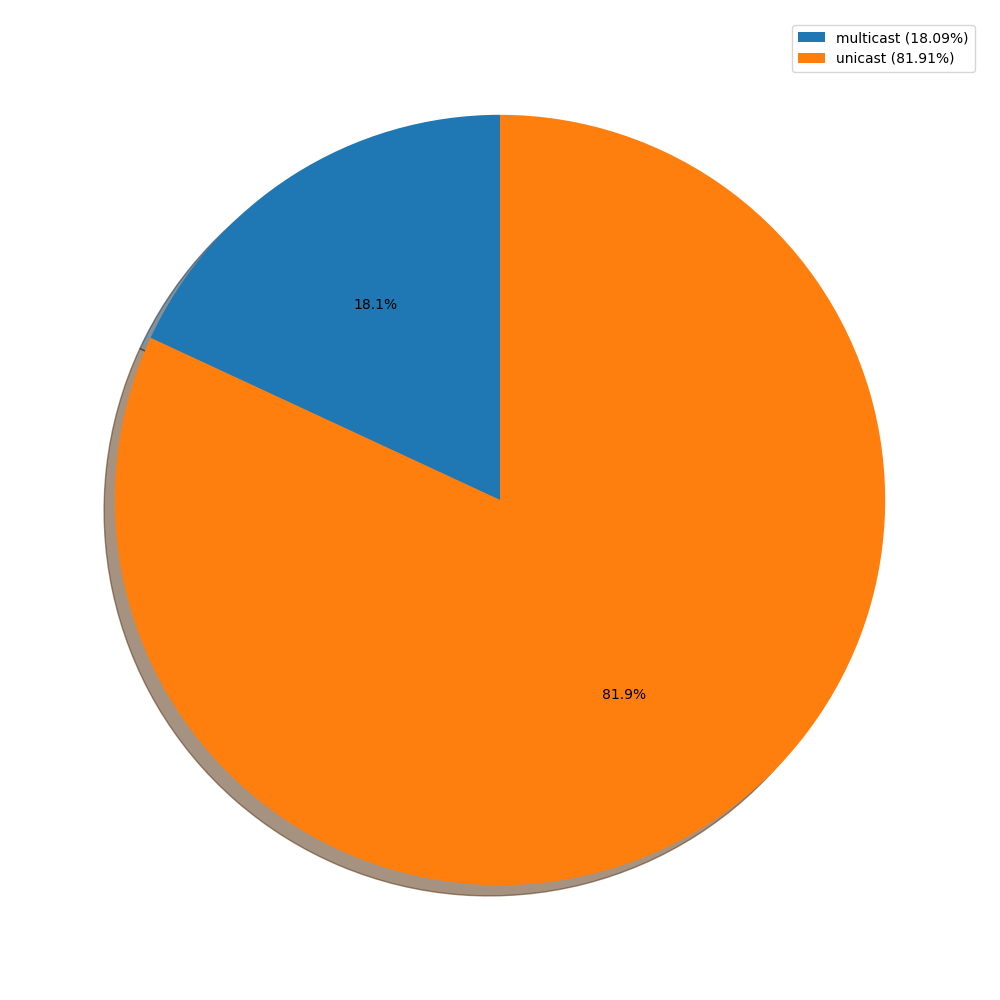
\includegraphics[scale=0.4]{../plots/trabajo_s1_probabilidades.png}
 \caption{Probabilidades de los simbolos de la fuente $S_1$ para la red de oficinas}
\end{figure}

\begin{figure}
 \centering
 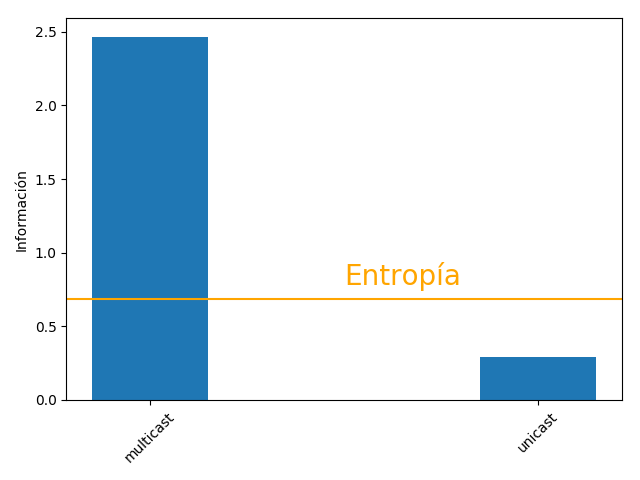
\includegraphics[scale=0.6]{../plots/trabajo_s1_informacion.png}
 \caption{Información de los simbolos de la fuente $S_1$ para la red de oficinas}
\end{figure}


Como se puede observar en ambos graficos el el simbolo 
destacado es el \textbf{unicast}, ya que este tiene mayor probabilidad
y menor cantidad de información. Esto nos dice que aproximadamente
sobre el cable el $81.91\%$ los paquetes fue unicast.
El sentido de esto puede deberse a que los únicos protocolos que
usan el tipo de mensajes broadcast son protocolos de control y representan
una pequeña proporcion del trafico total de la red.

\clearpage

\subsubsection{Fuente ARP}

\begin{figure}
\centering
 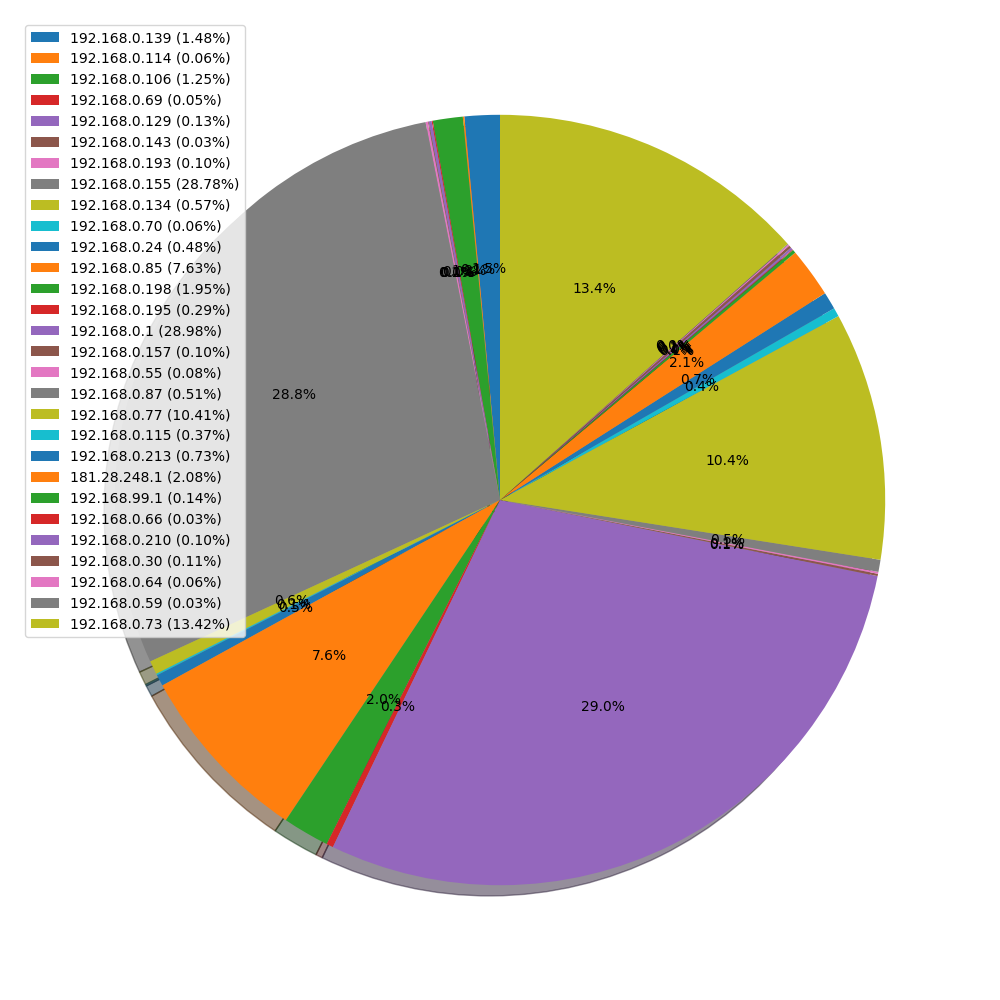
\includegraphics[scale=0.4]{../plots/trabajo_s2_probabilidades.png}
 \caption{Probabilidades de los simbolos de la fuente $S_2$ para la red de oficinas}
\end{figure}

\begin{figure}
 \centering
 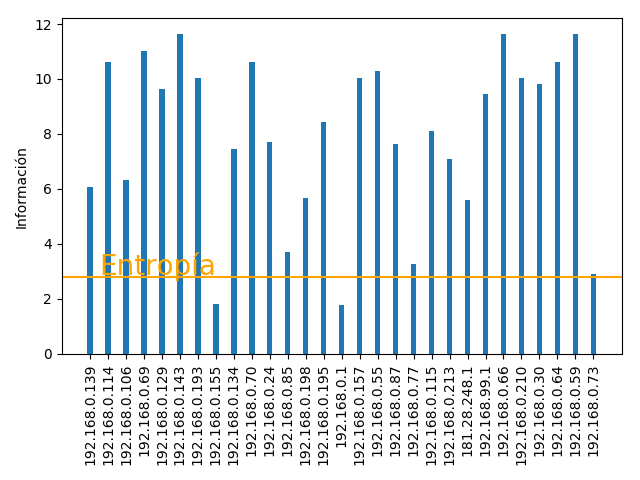
\includegraphics[scale=0.6]{../plots/trabajo_s2_informacion.png}
 \caption{Información de los simbolos de la fuente $S_2$ para la red de oficinas}
\end{figure}

En estos graficos se puede ver que efectivamente que el nodo \textbf{192.168.0.1}
es el destacado. Por previo conocimiento de la red se sabe que este
es el router lo cual refuerza nuestra hipotesis sobre los nodos destacados.
Tambien se observa que la entropía alcanzada es de $2.87$ cuando la máxima
es $4.85$ y por tanto $\eta_{C} = 0.41$

\clearpage
\subsubsection{Topolog\'ia de la Red}
\begin{center}
 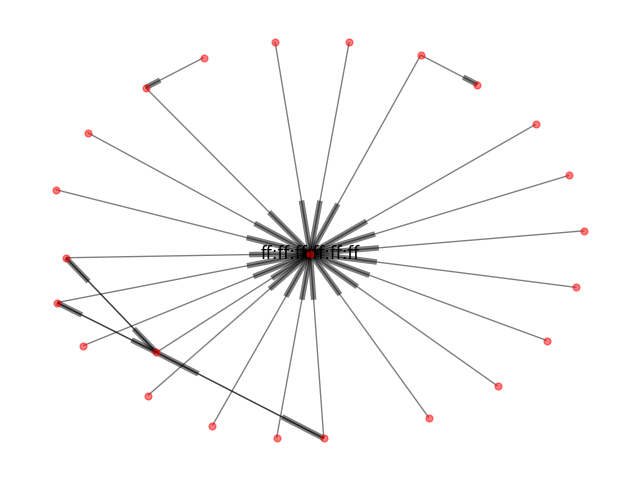
\includegraphics[scale=0.6]{../plots/trabajo_s2_topologia.png}
\end{center}

Se puede observar que la topogia de mensajes arp es de tipo estrella
y que el grafo es conexo. El nodo del centro resulta ser la MAC $ff:ff:ff:ff:ff:ff$
es decir los mensajes broadcast. Se puede ver que hay pocos nodos que le hayan
enviado un paquete arp a otro que no sea el broadcast. Esto se debe
a que al estar detrás de un switch, los mensajes unicast de respuesta (\textit{is-at})
no son forwardeados a la maquina que realizá la captura aun estando en modo promiscuo
la interfaz salvo que se trate de un mensaje unicast que responde la misma maquina que
hace la captura. Aun asi se filtran mensajes unicast de pc's a otras pc's. Esto como
se dijo puede deberse a switchs que no aprendieron bien la tabla de forwardeo.

\subsection{Experimento Tavo}

\subsubsection{Fuente Unicast-Multicast}

\hspace*{-1.5cm}
 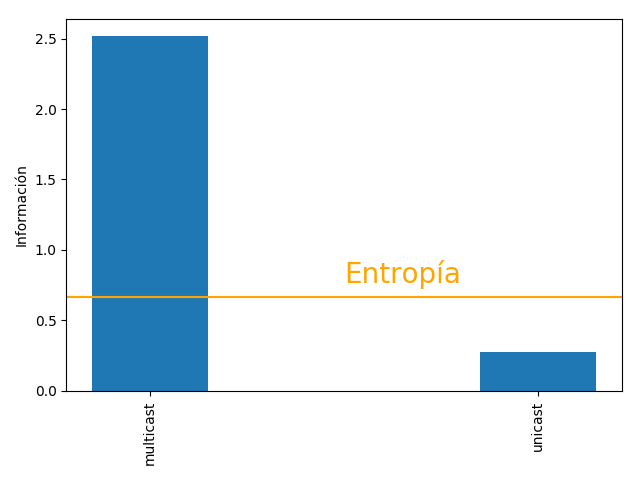
\includegraphics[scale=0.6]{../plots/labos_s1_informacion.png}
 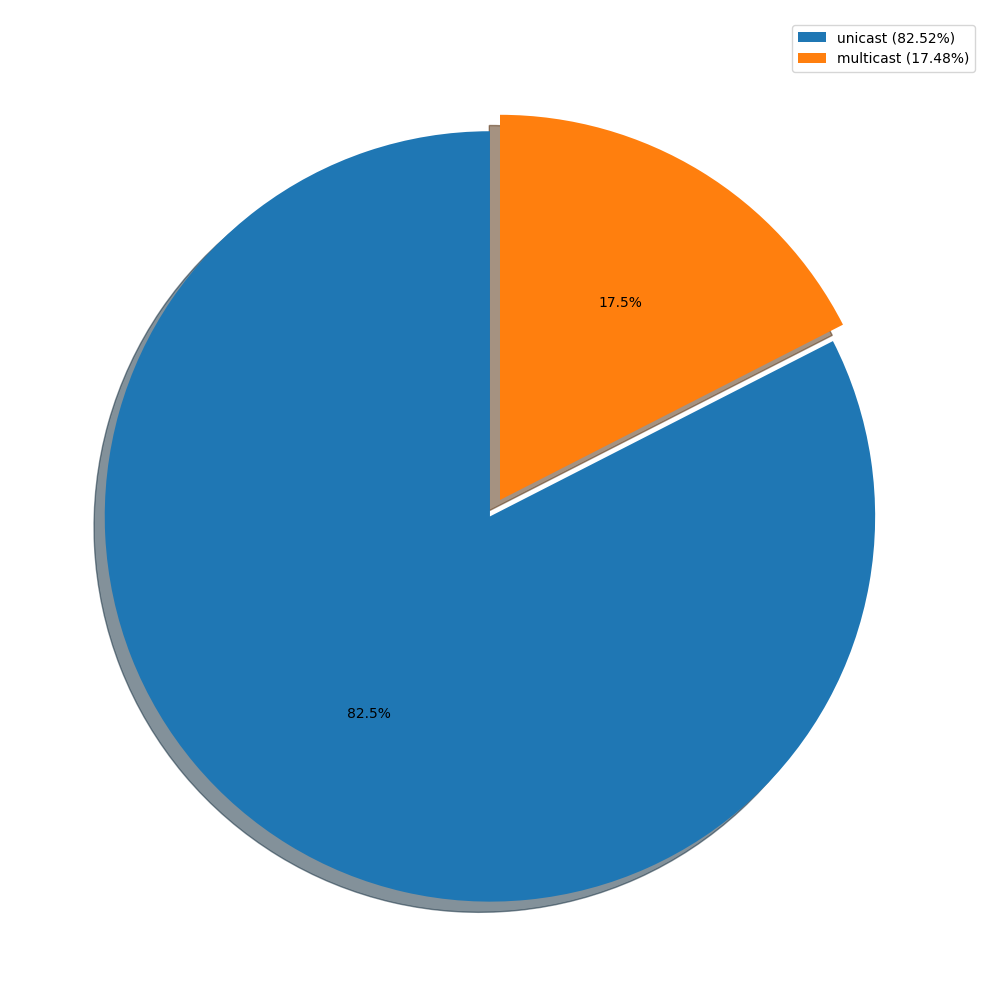
\includegraphics[scale=0.4]{../plots/labos_s1_probabilidades.png}

\subsubsection{Fuente ARP}

\hspace*{-1.5cm}
 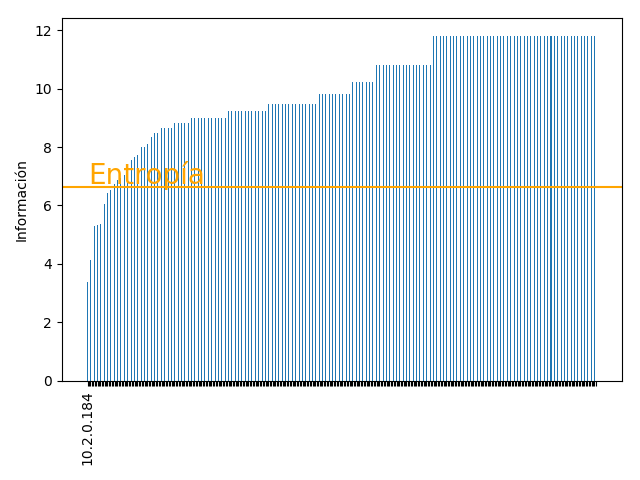
\includegraphics[scale=0.6]{../plots/labos_s2_informacion.png}
 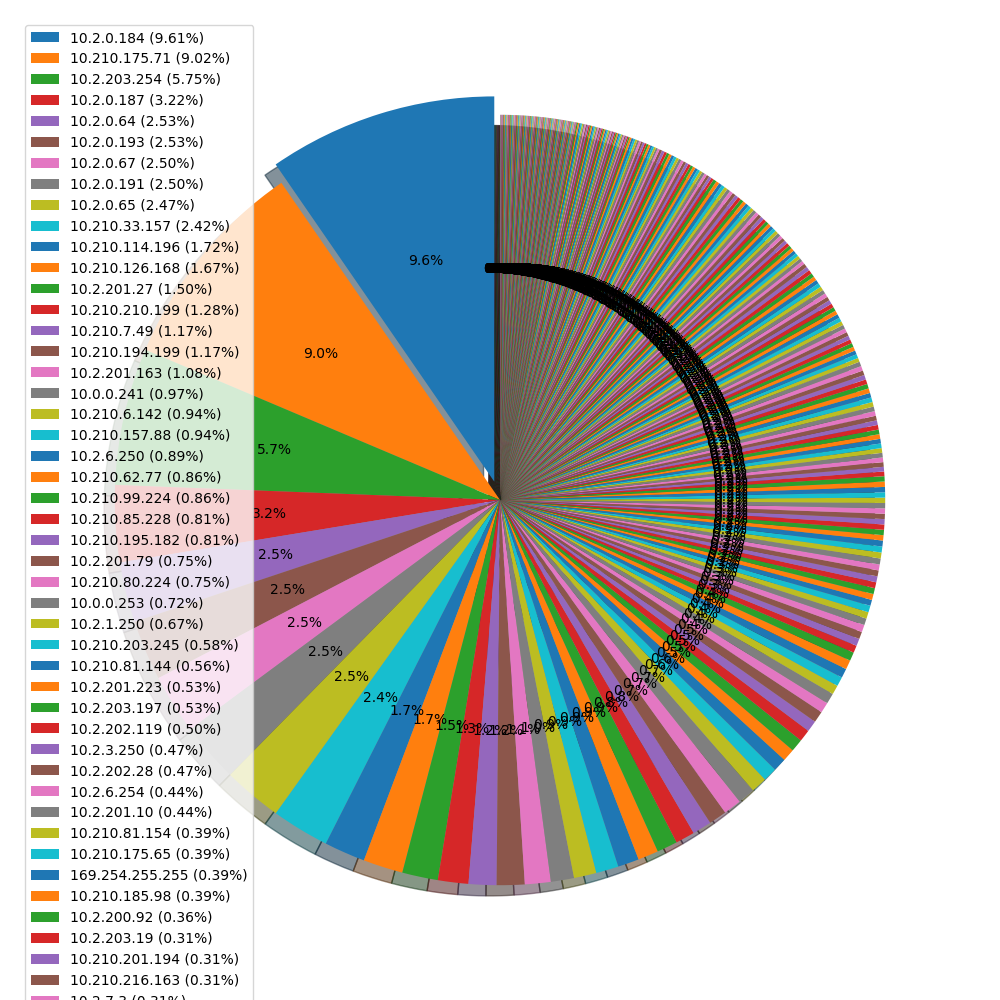
\includegraphics[scale=0.4]{../plots/labos_s2_probabilidades.png}

\subsubsection{Topolog\'ia de la Red}
\begin{center}
 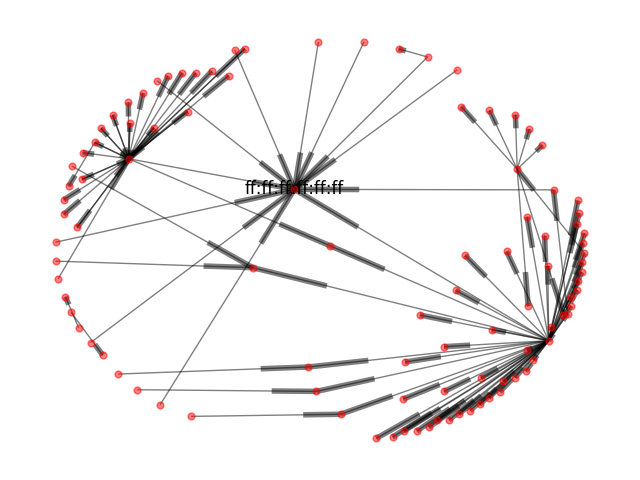
\includegraphics[scale=0.6]{../plots/labos_s2_topologia.png}
\end{center}

\begin{figure}
	\centering
	\begin{tabular}{|c|c|c|c|}
		\hline
		Red & Entropía & Entropía Max & $\eta_{C}$ \\
		\hline
		Hogareña & 2.034 & 2.807 & 0.380 \\
		\hline
		Oficinas & 2.777 & 4.858 & 0.750 \\
		\hline
		Laboratorio & 6.619 & 8.484 & 0.282 \\
		\hline
	\end{tabular}
	\caption{Entropía vs Max Entropía de las fuentes $S_2$ de las redes}
\end{figure}
